\section {Testing}
\paragraph{}
Testing was used to ensure the robustness of the solution, guaranteeing that all the project's objectives were met successfully. Recall that the tests themselves were designed in section 2, with the intention of being carried out after the design had been fully implemented, and were grouped by which objective each aimed to test.

\paragraph{}
The auditory nature of the program means it is not possible to fully provide evidence of successful tests with only the written word. Screenshots are therefore included within the document for the benefit of the reader, as well as external video links containing both video and audio.

\paragraph{}
Naturally testing would not be complete without checking for the presence of errors. Recall therefore that the design of tests encompasses both boundary and erroneous data in addition to "normal data", particularly in the loading of playlists and audio files.

\paragraph{}
Evidence for each test follows the same basic structure:
\begin{itemize}
	\item Re-cap of test
	\item Supplied test data
	\item Expected result
	\item Observed result
	\item Conclusion: was the observed result as expected?
\end{itemize}

\paragraph{}
For the benefit of the reader, a summary of the results of all tests is contained below.
Below that are the tests themselves, expanded in more detail.

\pagebreak
\subsection{Testing Summary}
{
	\renewcommand{\arraystretch}{1.5}
	\begin{table}[h!]
		\begin{center}
			\begin{tabularx}{1.0 \textwidth} {
					| >{\raggedright\arraybackslash}p{0.15\linewidth} 
					| >{\raggedright\arraybackslash}p{0.5\linewidth}
					| >{\raggedright\arraybackslash}X 
					|>{\raggedright\arraybackslash}p{0.15\linewidth}
					|
				}
				\hline
				Test Number & Description & Relevant Video Link (if any) & Passed \\
				
				\hline
				1.1 & The user must have the option to create a new playlist from a list of audio files on the system.  To test this, I will therefore place a variety of audio files on disk and verify they are detected by the program. Non-audio files will not be able to be selected, for obvious reasons. As the only audio file currently supported is the ".wav" format, any file without this extension will not be displayed. & N/A & Yes
				\\
				
				
				\hline
			\end{tabularx}
		\end{center}
	\end{table}
}

\pagebreak
\subsection{Test 1.1}
\subsubsection{Description}
\paragraph{}
{
	\centering
	\fbox{\begin{minipage}{15cm}
			"The user must have the option to create a new playlist from a list of audio files on the system.  To test this, I will therefore place a variety of audio files on disk and verify they are detected by the program. Non-audio files will not be able to be selected, for obvious reasons. As the only audio file currently supported is the ".wav" format, any file without this extension will not be displayed."
	\end{minipage}}
}

\subsubsection{Supplied Test Data}
\paragraph{}
A variety of audio files were placed inside the system's music folder. Some were hidden inside subfolders. In order to test the behaviour of erroneous data as described above, the music folder also contained an mp3 file, which is not supported currently.

\begin{figure}[H]
	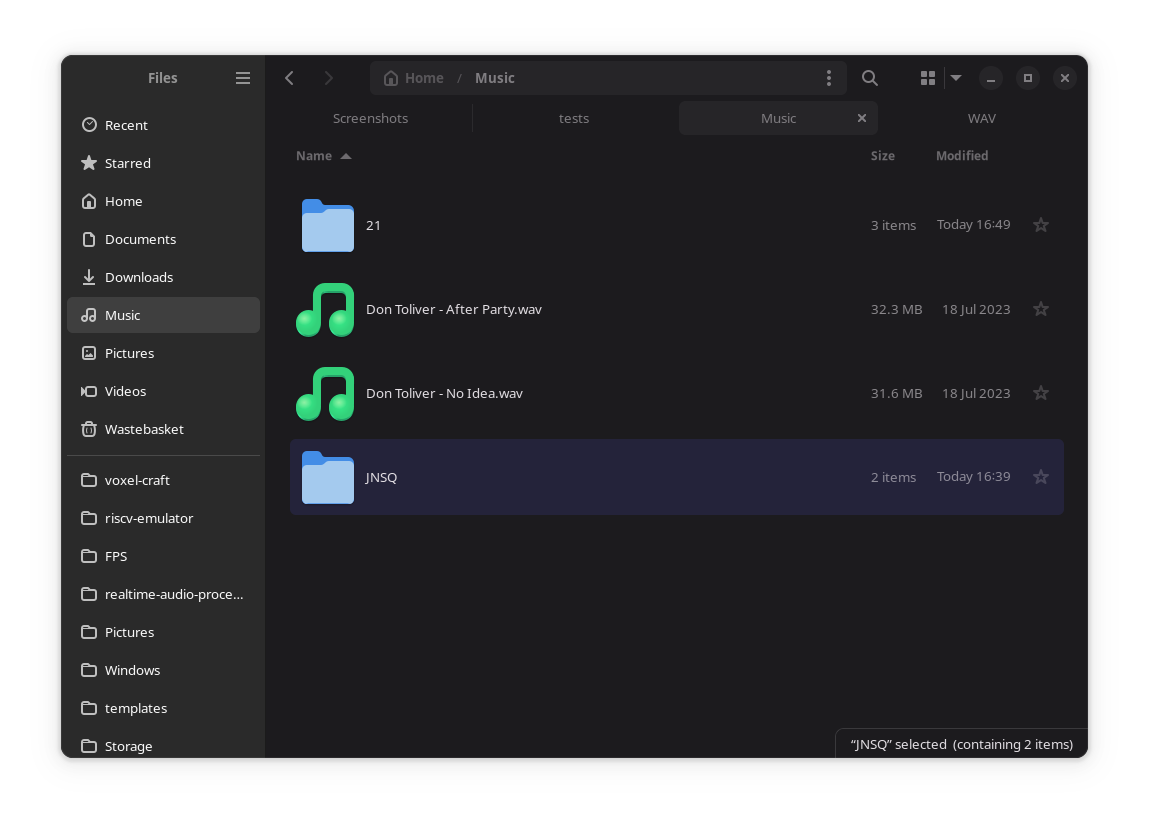
\includegraphics[width=14cm]{./tests/1.1.1.png}
\end{figure}
\begin{figure}[H]
	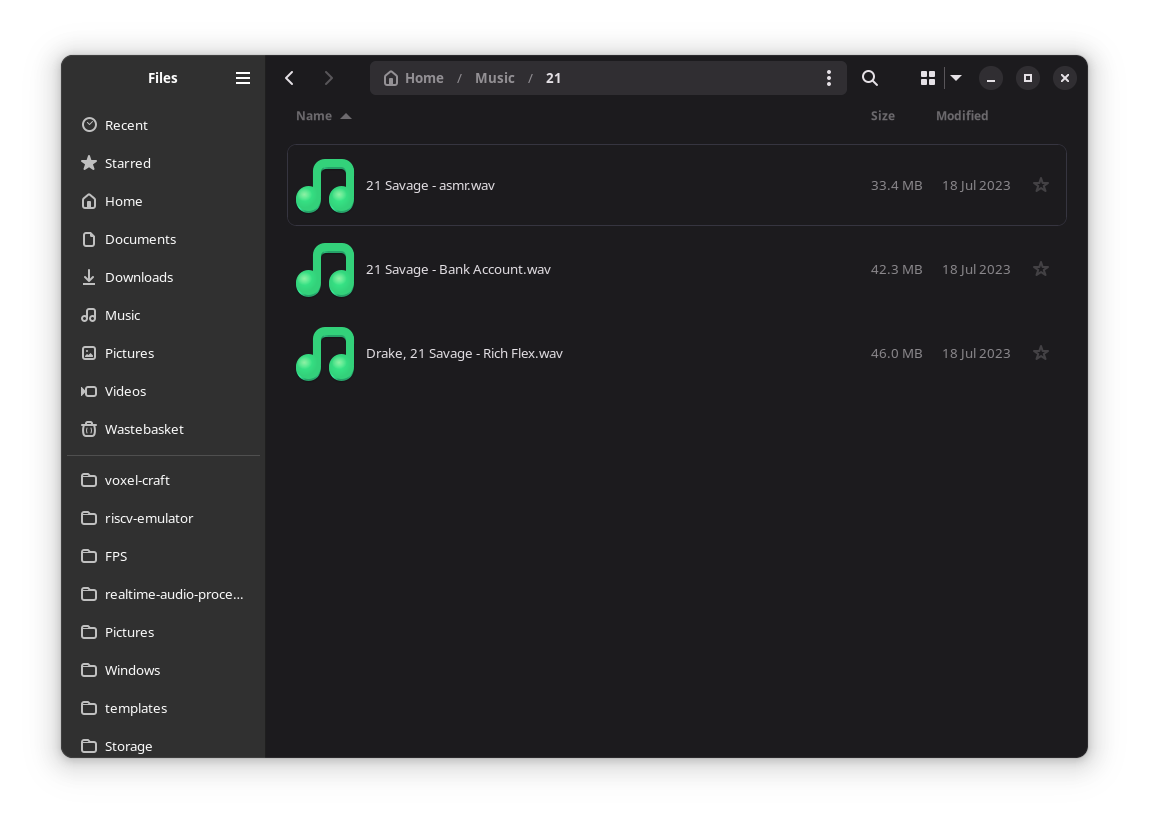
\includegraphics[width=14cm]{./tests/1.1.2.png}
\end{figure}
\begin{figure}[H]
	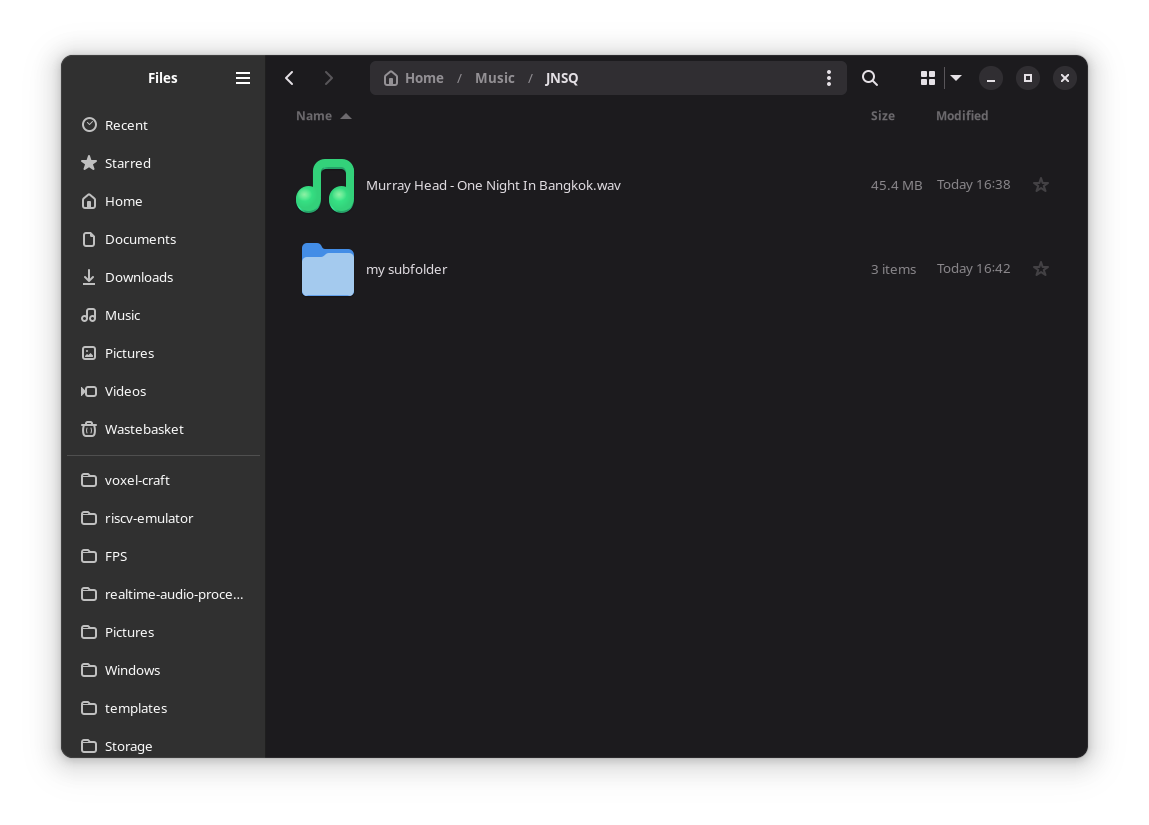
\includegraphics[width=14cm]{./tests/1.1.3.png}
\end{figure}
\begin{figure}[H]
	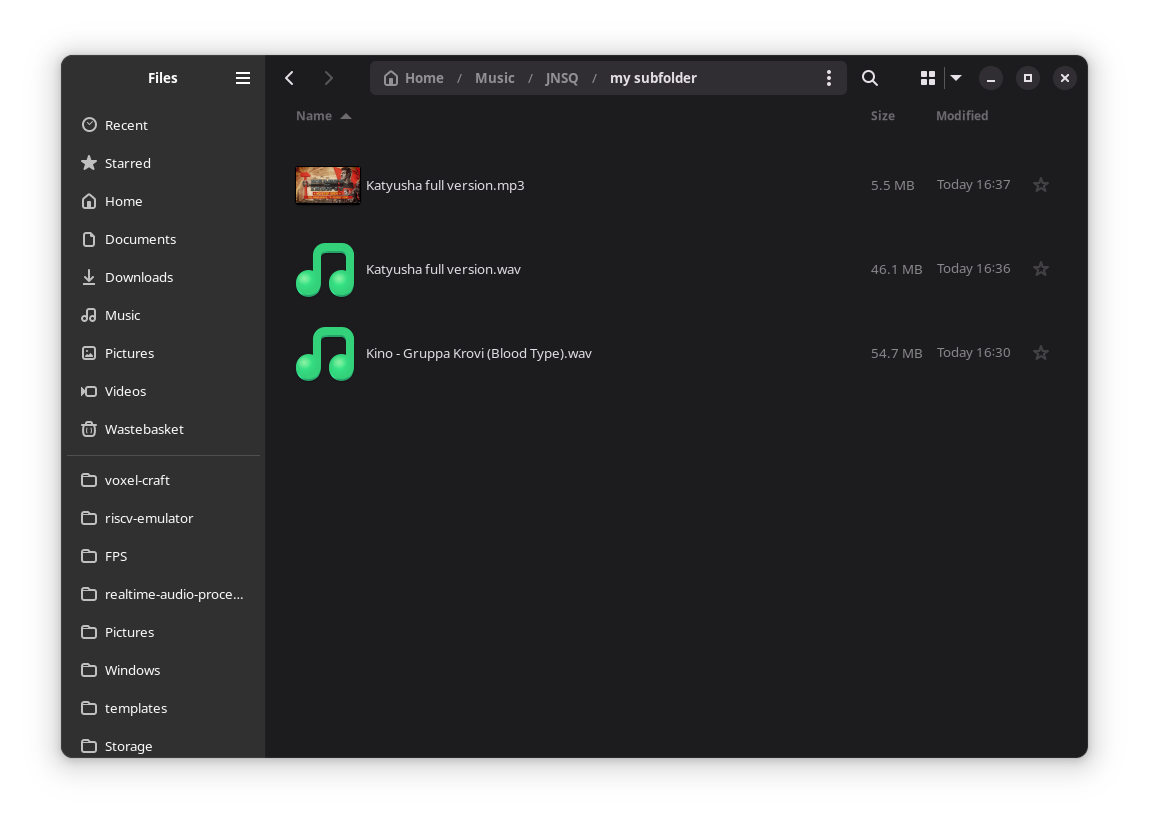
\includegraphics[width=14cm]{./tests/1.1.4.png}
\end{figure}
\begin{figure}[H]
	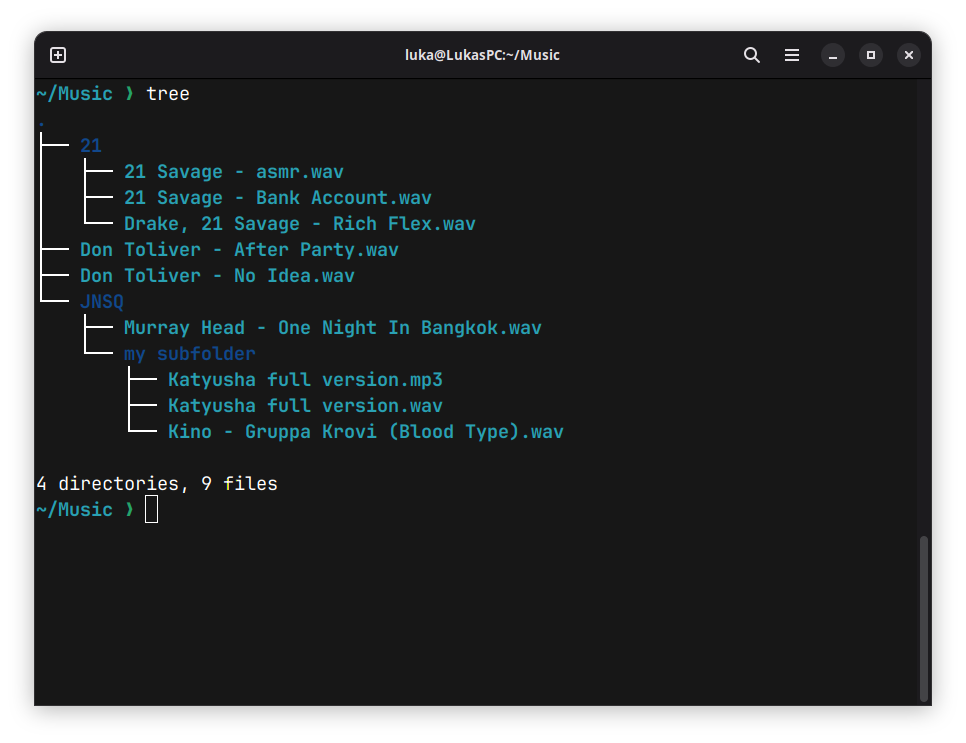
\includegraphics[width=14cm]{./tests/1.1.5.png}
	\caption{Terminal output that summarises filesystem structure}
\end{figure}

\subsubsection{Expected Result}
The program should detect all the ".wav files", but not any other files, such that the ".mp3 file" is not detected. All detected files should be displayed within the GUI.

\subsubsection{Observed Result}
\begin{figure}[H]
	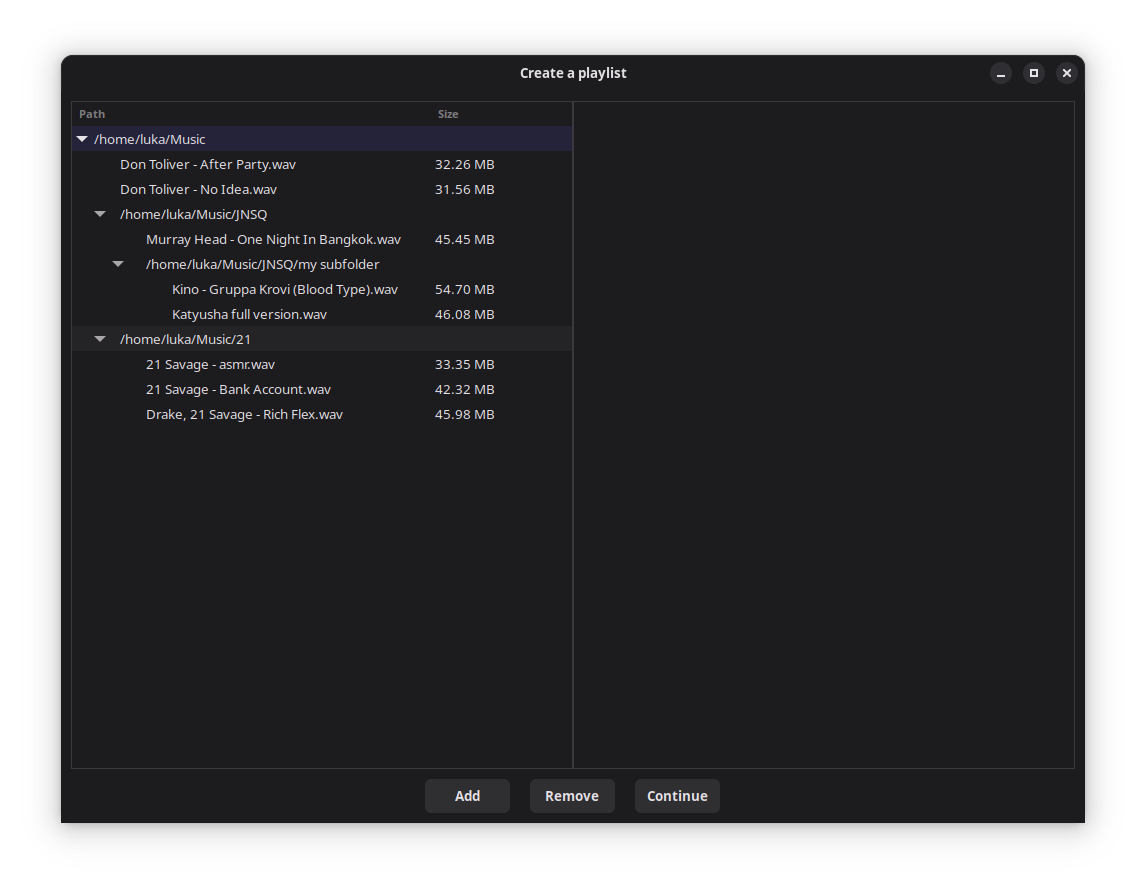
\includegraphics[width=14cm]{./tests/1.1.6.png}
	\caption{Program GUI output. All WAV files have been detected and displayed, but the mp3 has not been. Files have been detected, even when they are inside subfolders.}
\end{figure}

\subsubsection{Conclusion}
This test passed, as all ".wav" audio files were detected, whilst other files were ignored, and the GUI displayed this appropriately.


\pagebreak
\subsection{Test 1.2}
\subsubsection{Description}
\paragraph{}
{
	\centering
	\fbox{\begin{minipage}{15cm}
			"I will then test if playlists created in the program can be successfully saved to disk, then loaded back into the program in a sanitised manner. In other words, playlists consisting solely of files which actually exist on disk should be loaded without error (such that audio playback starts), but playlists with non-existent audio files should fail to load and notify the user of the error."
	\end{minipage}}
}

\subsubsection{Supplied Test Data}
\paragraph{}
The test was split into two parts - the first would be attempting to create, save, then load a playlist in which all audio files existed. For the first part of this test, the same selection of files was used as in test 1.1. For the second part of the test, the playlist was to be modified after its creation by appending the following non-existent file to the end of it:
\textit{/this/audio/files/does/not/exist.wav}
\begin{figure}[H]
	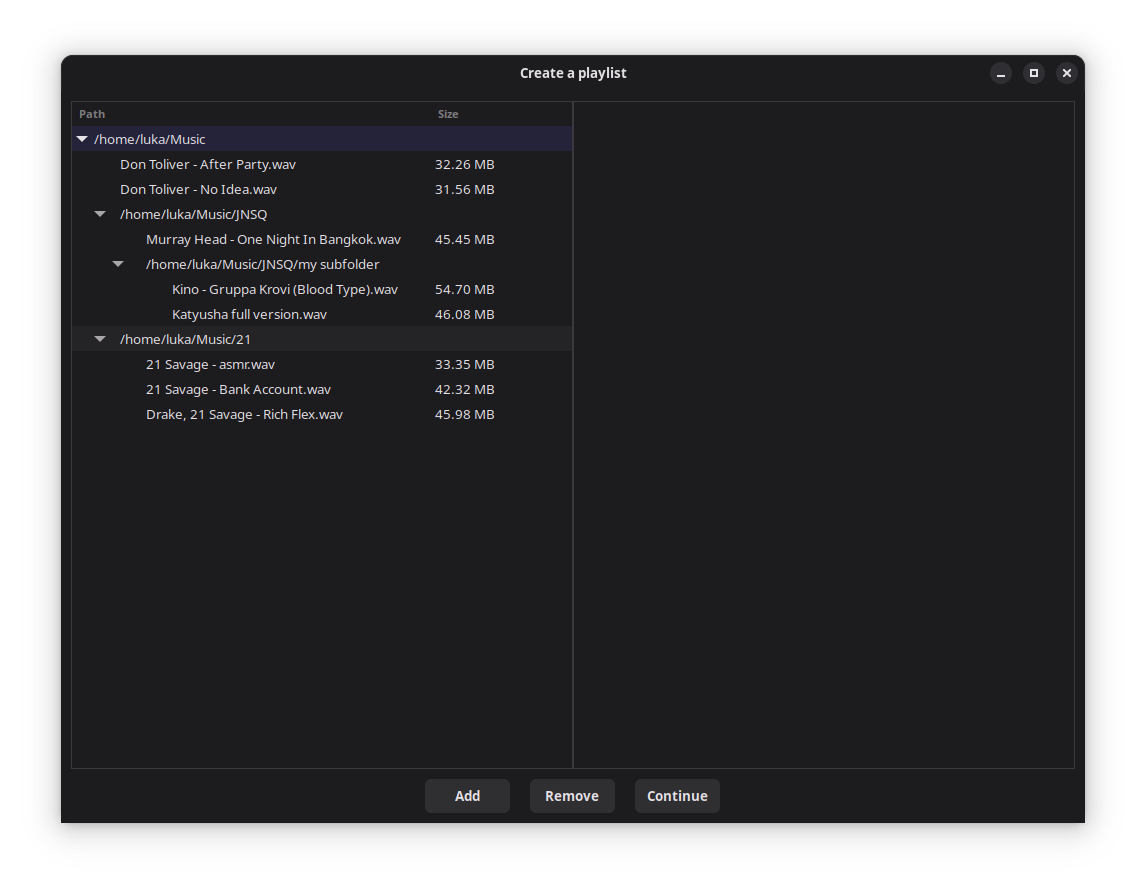
\includegraphics[width=14cm]{./tests/1.1.6.png}
	\caption{Files from test 1.1, which should be turned into a playlist then saved and loaded back}
\end{figure}

\subsubsection{Expected Result}
The user should be able to use the GUI to add all files to a playlist, which is then saved successfully to disk. The user should then be able to load this playlist to begin audio playback. This should succeed. However, when the playlist is modified to include a file that no longer exists, the program should raise an error and refuse to load the playlist.

\subsubsection{Observed Result}
Video evidence was recorded for the test, which can be viewed \href{https://drive.google.com/file/d/1yGeMYYI9ts37JsoA_9agpKTGBL0s8Dms/view?usp=sharing}{here}\footnote{
	https://drive.google.com/file/d/1yGeMYYI9ts37JsoA\_9agpKTGBL0s8Dms/view?usp=sharing
}.  The video shows a user created a valid playlist, then saving it to disk. He then loads the playlist into the program and audio playback successfully starts. He then restarts the program and attempts to load the playlist again, after modifying it by adding an invalid file path. The program refuses to load this invalid playlist.

\subsubsection{Conclusion}
The program successfully created, saved, then loaded the valid playlist but refused to load the invalid playlist, such that the test passed.

\pagebreak
\subsection{Test 1.3}
\subsubsection{Description}
\paragraph{}
{
	\centering
	\fbox{\begin{minipage}{15cm}
			"After loading a playlist and beginning audio playback, the audio files contained within must appear alphabetically in the audio file selection screen, ordered in ascending order by their respective filenames."
	\end{minipage}}
}

\subsubsection{Supplied Test Data}
A new playlist was again created. It was deemed suitable as it contained audio files starting with upper case letters, lower case letters, and even numbers, hence allowing for all reasonable combinations of alpha-numeric values to be covered.
\begin{figure}[H]
	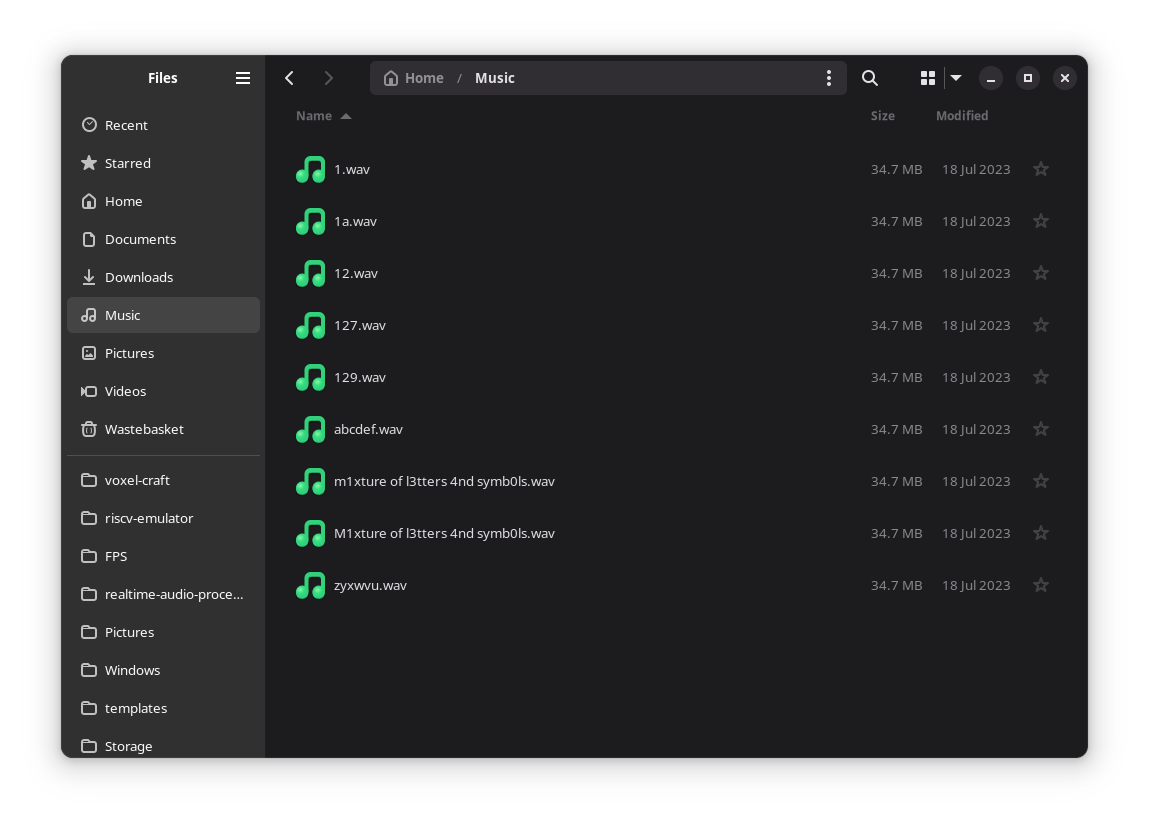
\includegraphics[width=14cm]{./tests/1.3.1.png}
\end{figure}

\subsubsection{Expectation}
\paragraph{}
When selecting a new audio file from the playlist (by going to \textit{File, Select Song}), the GUI should organise them alphabetically by their filenames. Numbers should come before letters, and the numbers should be ordered too (e.g, 1, 2, 3...). Lower case versions of the same letter should come before upper case versions (as they appear first in ASCII ordering).
\paragraph{}
Hence the expected order for display is as follows:
\begin{enumerate}
	\item 1.wav
	\item 1a.wav
	\item 12.wav
	\item 127.wav
	\item 129.wav
	\item abcdef.wav
	\item m1xture of l3tters 4nd symb0ls.wav
	\item M1xture of l3tters 4nd symb0ls.wav
	\item zyxwvu.wav
\end{enumerate}

\subsubsection{Observed Result}
The observed result was as follows:
\begin{figure}[H]
	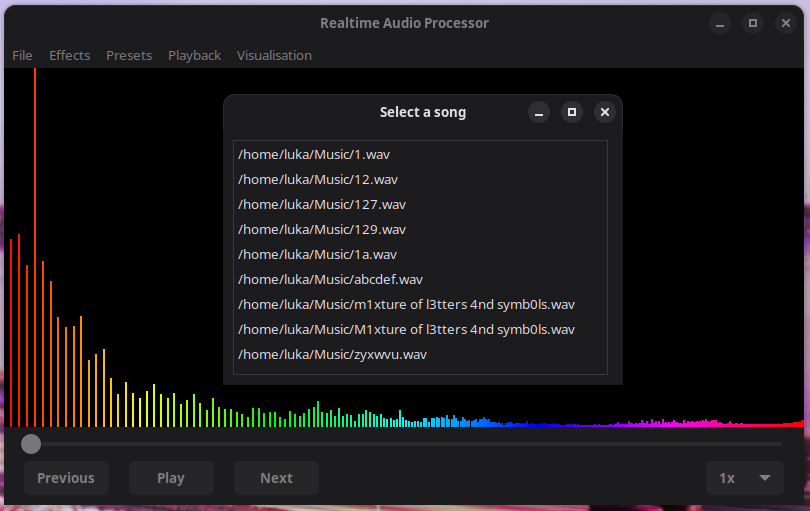
\includegraphics[width=14cm]{./tests/1.3.2.png}
\end{figure}

\subsubsection{Conclusion}
The observed result and expected result were identical, such that the test passed.


\pagebreak
\subsection{Test 1.4}
\subsubsection{Description}
\paragraph{}
{
	\centering
	\fbox{\begin{minipage}{15cm}
			"Any invalid audio files should be skipped over, and should not crash the program. The user should be notified if this happens."
	\end{minipage}}
}

\subsubsection{Supplied Test Data}
A new playlist was again created, containing three files. The first and last files were valid audio files, but the middle one was corrupt. The playlist contained these three files:
\begin{figure}[H]
	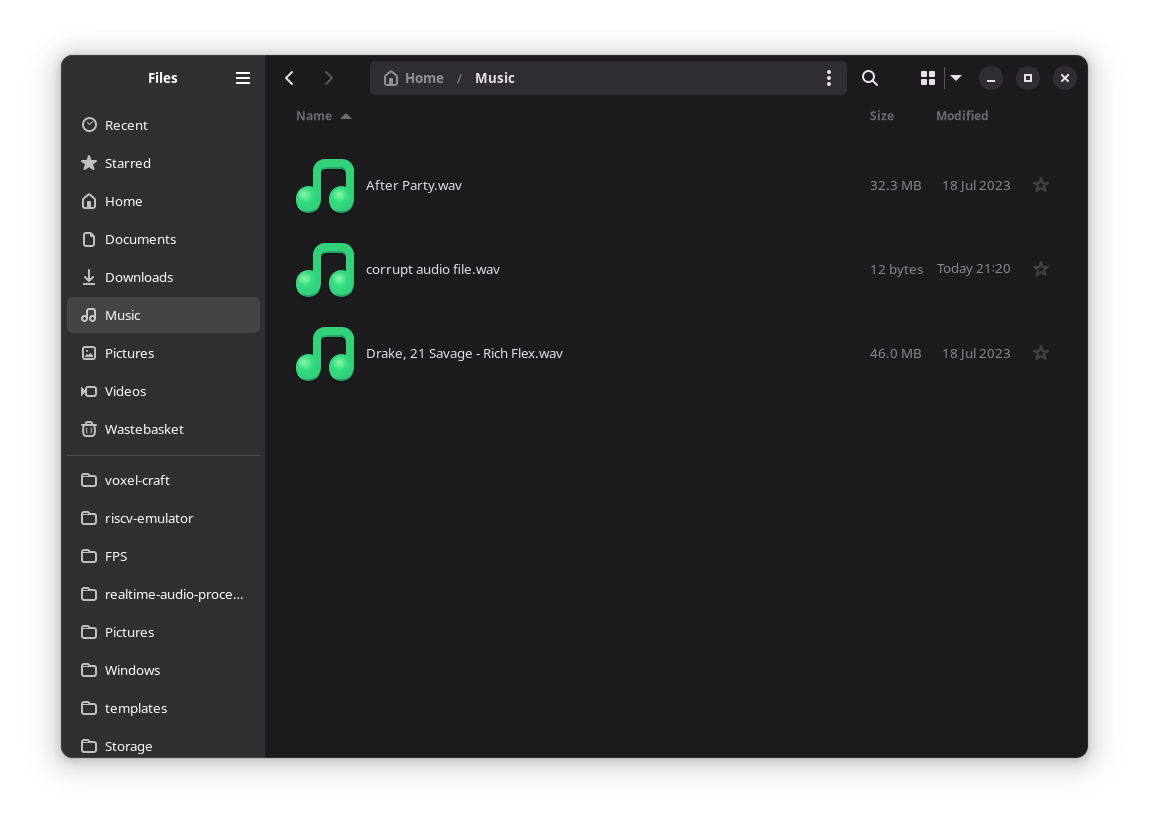
\includegraphics[width=14cm]{./tests/1.4.1.png}
\end{figure}

\subsubsection{Expectation}
\paragraph{}
The program should initially begin audio playback correctly when it loads the first audio file. However, when the next audio file (which is corrupt) is to be loaded by the program, it should fail, and the program should notify the user of the error. This corrupt file should then be skipped, and playback should resume with the third audio file.
 
\subsubsection{Observed Result}
Video evidence was recorded for the test, which can be viewed \href{https://drive.google.com/file/d/1IWSDFYTCctY-Voe49W1-w-7M0zj7ucMX/view?usp=sharing}{here}\footnote{
	https://drive.google.com/file/d/1IWSDFYTCctY-Voe49W1-w-7M0zj7ucMX/view?usp=sharing
}.  The video shows a user loading the testing playlist, in which audio playback starts. They then skip to the end of the song, waiting for it to finish. When it does, the program attempts to load the next audio file (which the reader will recall is invalid). Naturally, the program catches this and raises an error to the user. This corrupt audio file is then skipped, and playback resumes with the next audio file.

\subsubsection{Conclusion}
The observed result and expected result were identical, such that the test passed.

\pagebreak
\subsection{Test 2.1}
\subsubsection{Description}
\paragraph{}
{
	\centering
	\fbox{\begin{minipage}{15cm}
			"A correct visualisation of a sine wave is apparent at 500 Hz, with a single peak corresponding to that frequency."
	\end{minipage}}
}

\subsubsection{Supplied Test Data}
An audio file consisting of a single sine wave at 500 Hz was generated using the popular audio editing program Audacity.

\subsubsection{Expected Result}
A single peak should be observed in the audio visualiser, towards the left of the screen, representing 500 Hz.

\subsubsection{Observed Result}
\begin{figure}[H]
	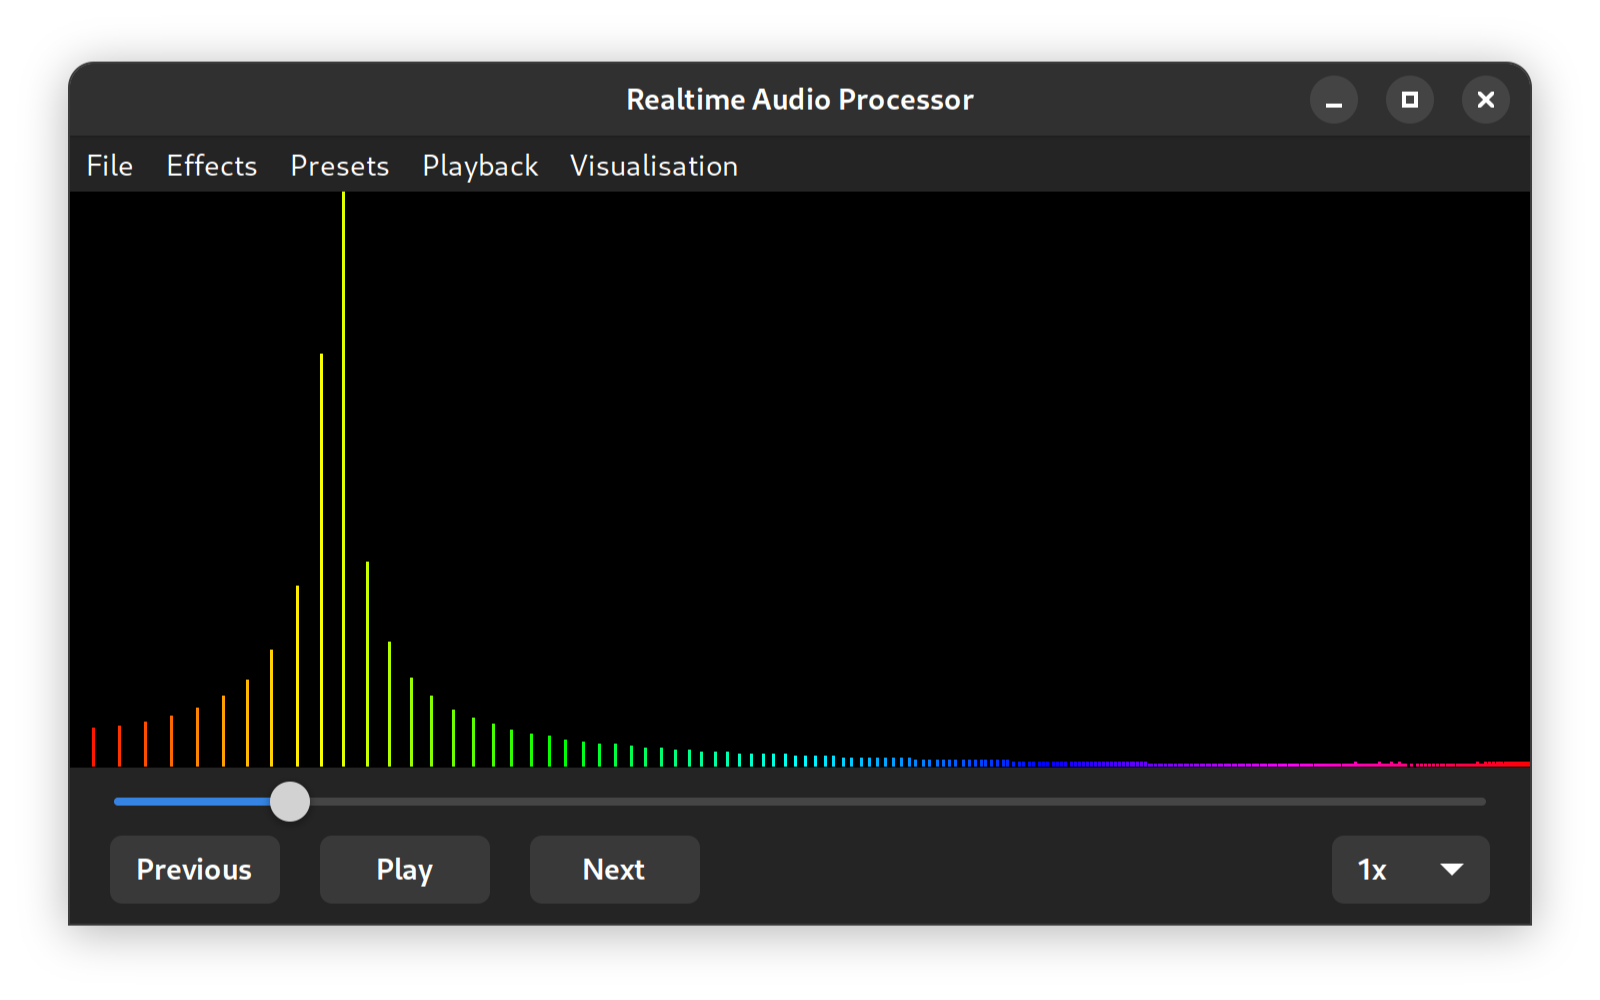
\includegraphics[width=14cm]{./tests/2.1.png}
\end{figure}

\subsubsection{}
A correct visualisation was achieved. The test was successful.

\pagebreak
\subsection{Test 2.2}
\subsubsection{Description}
\paragraph{}
{
	\centering
	\fbox{\begin{minipage}{15cm}
			"A correct visualisation of a sine wave is apparent at 1,000 Hz, with a single peak corresponding to that frequency."
	\end{minipage}}
}

\subsubsection{Supplied Test Data}
An audio file consisting of a single sine wave at 1,000 Hz was generated using the popular audio editing program Audacity.

\subsubsection{Expected Result}
A single peak should be observed in the audio visualiser, to the right of the peak observed in Test 1.1 (as the frequency is higher).

\subsubsection{Observed Result}
\begin{figure}[H]
	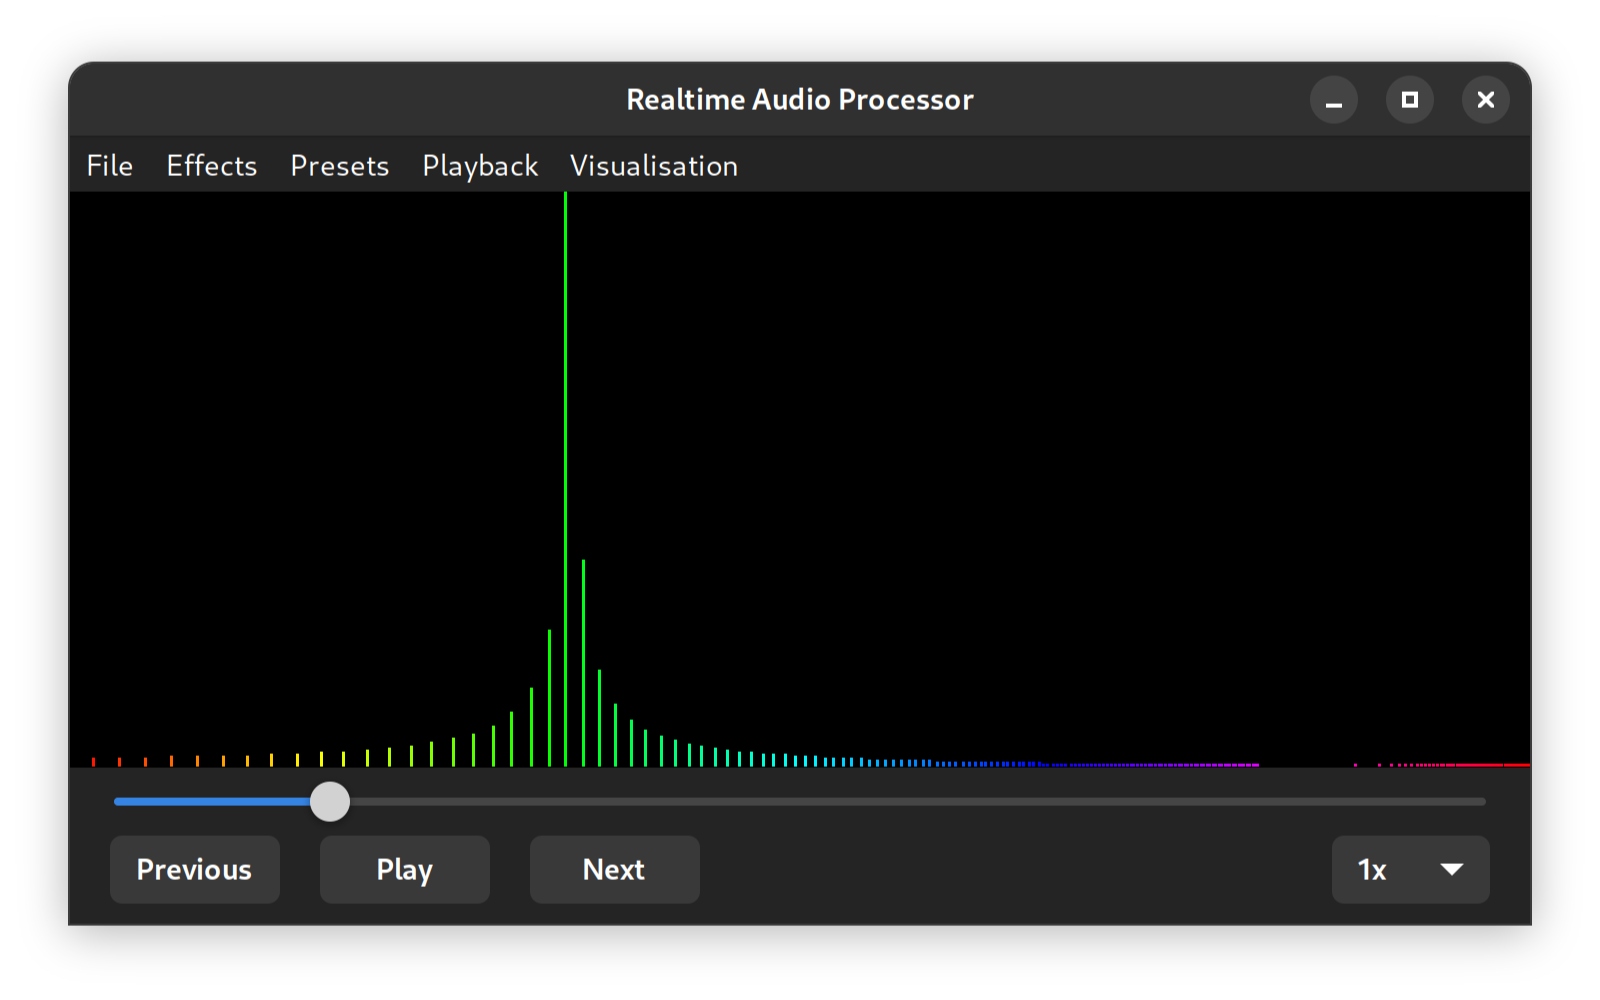
\includegraphics[width=14cm]{./tests/2.2.png}
\end{figure}

\subsubsection{}
A correct visualisation was achieved. The test was successful.

\pagebreak
\subsection{Test 2.3}
\subsubsection{Description}
\paragraph{}
{
	\centering
	\fbox{\begin{minipage}{15cm}
			"Sine waves outside the human audible range, at 10 Hz and 30,000 Hz respectively, produce no visible output, as they are inaudible."
	\end{minipage}}
}

\subsubsection{Supplied Test Data}
An audio file consisting of two sine waves (at 10 Hz and 30,000 Hz respectively) was generated using the popular audio editing program Audacity.

\subsubsection{Expected Result}
The input audio is completely inaudible, so there should be no output in the visualiser.

\subsubsection{Observed Result}
\begin{figure}[H]
	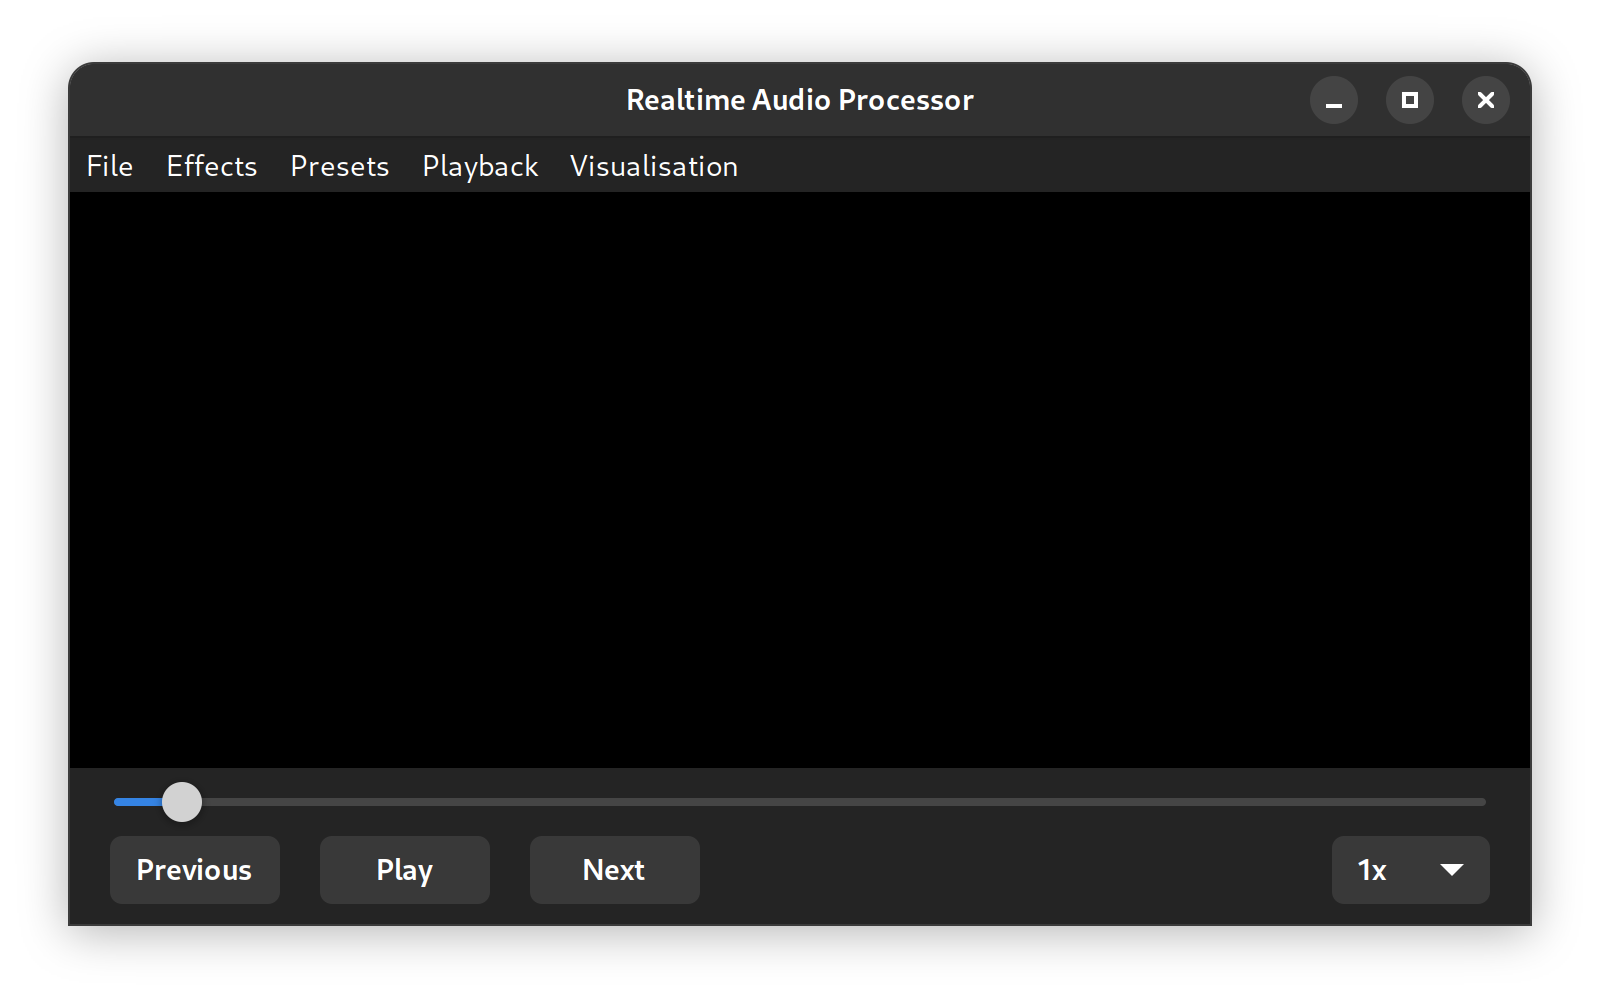
\includegraphics[width=14cm]{./tests/2.3.png}
\end{figure}

\subsubsection{}
A correct visualisation was achieved. The test was successful.

\pagebreak
\subsection{Test 2.4}
\subsubsection{Description}
\paragraph{}
{
	\centering
	\fbox{\begin{minipage}{15cm}
			"A correct visualisation of two sine waves (one at 1,000 Hz and one at 10,000 Hz) is apparent, with two separate peaks corresponding to those frequencies."
	\end{minipage}}
}

\subsubsection{Supplied Test Data}
An audio file consisting of two sine waves (at 1,000 Hz and 10,000 Hz respectively) was generated using the popular audio editing program Audacity.

\subsubsection{Expected Result}
The visualiser should display two peaks, one to the right of the other. Recall that the x-axis is non-linear as it uses the Bark scale, so they will not be a "linear" distance apart.

\subsubsection{Observed Result}
\begin{figure}[H]
	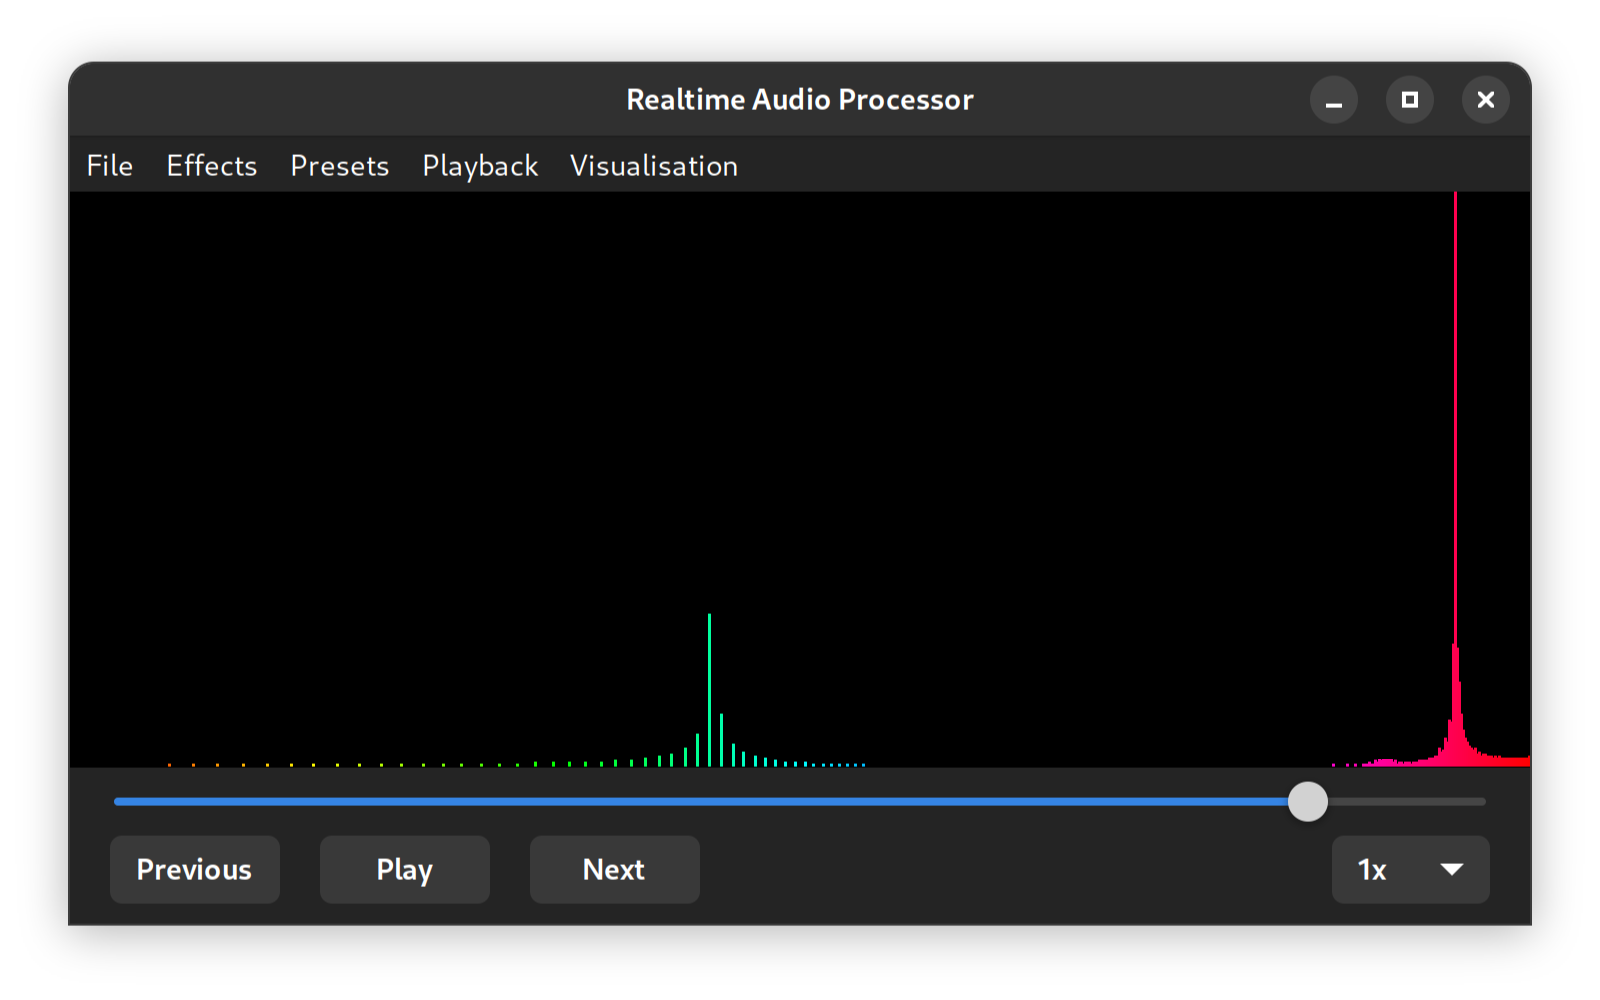
\includegraphics[width=14cm]{./tests/2.4.png}
\end{figure}

\subsubsection{}
A correct visualisation was achieved. The test was successful.


\pagebreak
\subsection{Test 2.5}
\subsubsection{Description}
\paragraph{}
{
	\centering
	\fbox{\begin{minipage}{15cm}
			"A correct visualisation of three sine waves (1,000 Hz, 5,000 Hz and 15,000 Hz ) is apparent, with three separate peaks corresponding to those frequencies."
	\end{minipage}}
}

\subsubsection{Supplied Test Data}
An audio file consisting of three sine waves (at 1,000 Hz and 5,000 Hz and 15,000 Hz respectively) was generated using the popular audio editing program Audacity.

\subsubsection{Expected Result}
The visualiser should display three peaks in successive order. Recall that the x-axis is non-linear as it uses the Bark scale, so they will not be a "linear" distance apart.

\subsubsection{Observed Result}
\begin{figure}[H]
	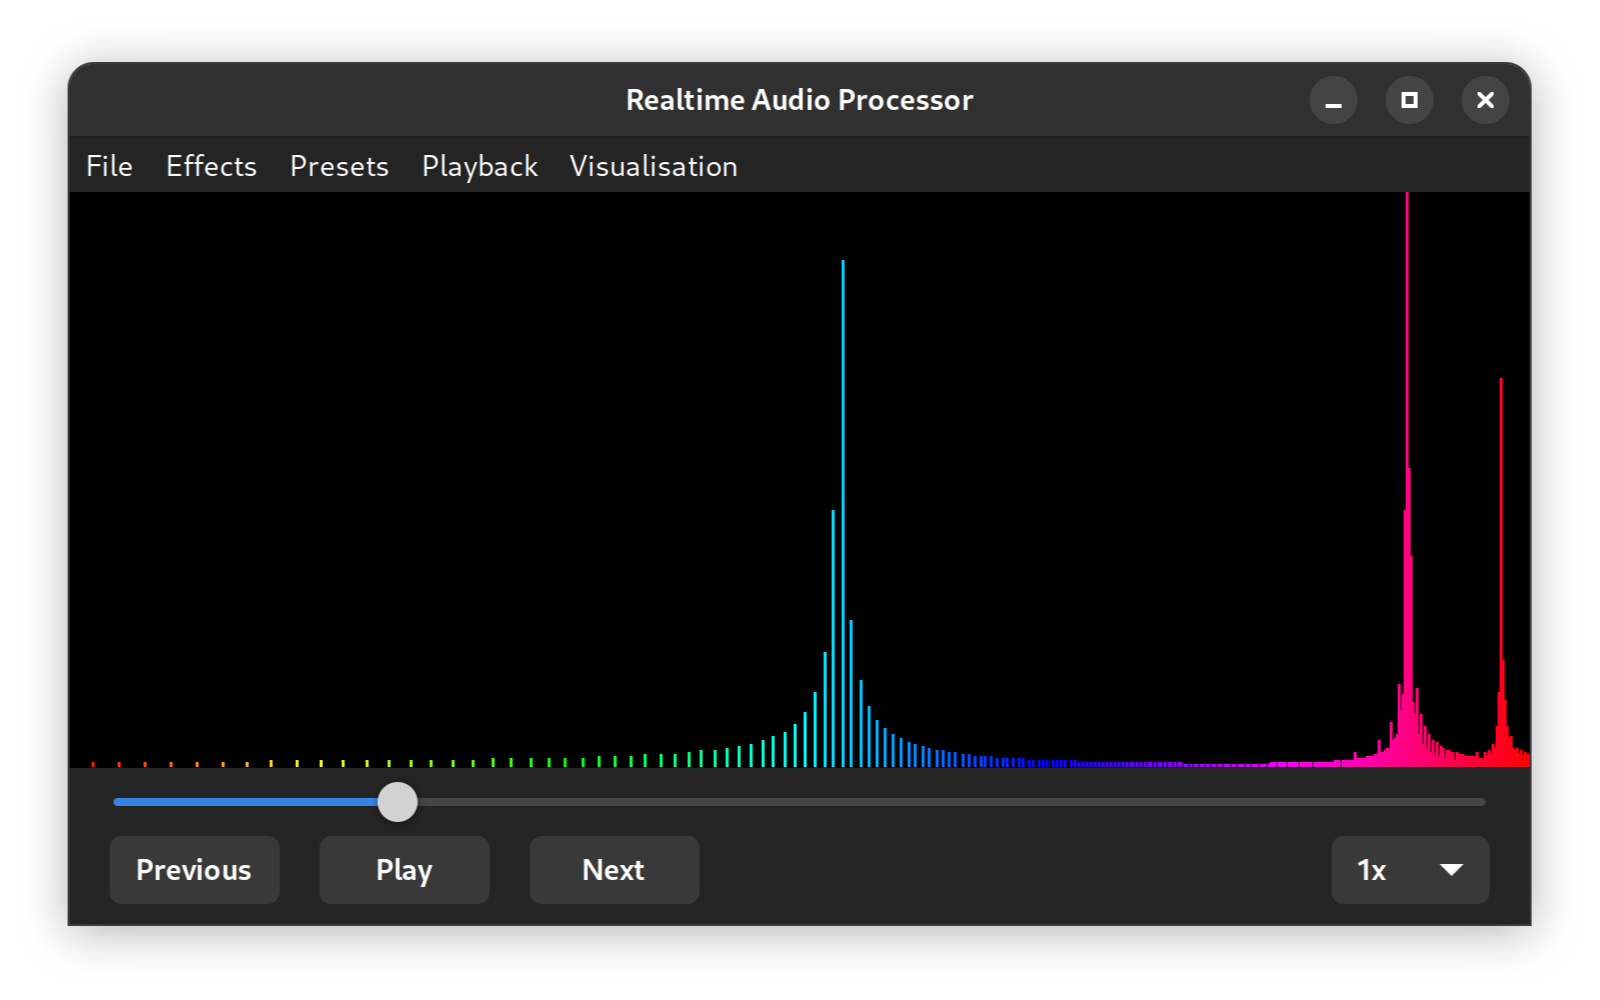
\includegraphics[width=14cm]{./tests/2.5.png}
\end{figure}

\subsubsection{}
A correct visualisation was achieved. The test was successful.